\documentclass{article}
\usepackage[margin=1in]{geometry}
\usepackage{microtype}
\usepackage{setspace}
\usepackage{amsmath}
\usepackage{parskip}
\usepackage{amssymb}
\usepackage{graphicx}

\graphicspath{{../public/}}

\parskip=4ex
\date{}
\author{}

\title{12.4 Application of Double Integrals}

\begin{document}
    \maketitle

    \textbf{Introduction}\\
    Imagine a lamina with variable density and suppouse said lamina occupies a region $ D $ of the region $ xy $ plane and its density (in units of mass per unit area) at a point $ (x,y) $ in $ D $ is given by $ Q(x,y) $, where $ Q $ is a continuous function on $ D $. This means that
    \[
        Q(x,y) = \lim \frac{\Delta m}{\Delta A} 
    \]

    where $ \Delta m ~\&~ \Delta A $ are the mass and area of a small ectangle that contains $ (x,y) $ and the limit is taken as the dimensions of the rectangle approach $ 0 $.
    
    \begin{center}
        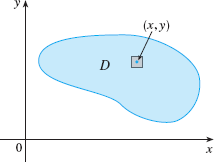
\includegraphics[width=6cm]{12_4_1}
    \end{center}

    To find the total mass $ m $ of the lamina, a rectangle $ R $ that contains $ D $ is divided into subrectangles $ R_{ij}  $ and consider $ Q(x,y) $ to be $ 0 $ outide $ D $. By choosing a point $ (x^{*}_{ij},y^{*}_{ij}) $ in $ R_{ij} $, then the mass of the part of the lamina occupying $ R_{ij} $ is approximately $ \rho(x^{*}_{ij},y^{*}_{ij}) \Delta A_{ij} $, where $ \Delta A_{ij} $ is the area of $ R_{ij} $. By adding all such masses, an approximation of the total mass is obtained.
    \[
      m \approx \sum^{k}_{i=1} \sum^{l}_{j=1} \rho(x^{*}_{ij},y^{*}_{ij}) \Delta A_{ij}  
    \]

    \begin{center}
        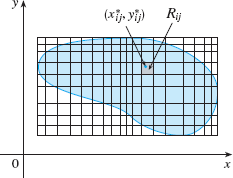
\includegraphics[width=6cm]{12_4_2}
    \end{center}

    By taking the finer partitions using smaller rectangles, the total mass $ m $ of the lamina is obtained through the limit of our summation.
    \[
      m = \lim_{\text{max } \Delta x_{i} , \Delta y_{j} \to 0}{\sum^{k}_{i=1} \sum^{l}_{j=1} \rho(x^{*}_{ij},y^{*}_{ij}) \Delta A_{ij} } = \iint_{D} \rho(x,y) ~dA 
    \]
    
   Other types of density are treated in the same manner by physicists. AN example would be an electric charge distrubuted over a region $ D $ and the charge desnity (in units of charge per unit area)is given by $ \sigma(x,y) $ at a point $ (x,y) $ in $ D $, then the total charge $ Q $ is given by
   \[
       Q = \iint_D \sigma(x,y)~dA
   \]

   \textbf{Ex 1}\\
   Charge is distributed over the triangular region $ D $ in the figure below so that the cahrge density at $ (x,y) $ is $ \rho(x,y)=xy $, measured in coulombs per square meter $ C/m^{2} $. Find the total charge.

   \begin{center}
       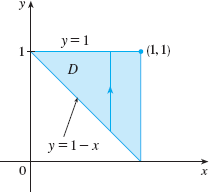
\includegraphics[width=6cm]{12_4_3}
   \end{center}

   \[
       \begin{gathered}
       Q = \iint_D \rho(x,y) ~dA = \int^{1}_{0} \int^{1}_{1-x} xy ~ dydx\\
       \int^{1}_{0} \text{\large{[}} x\frac{y^{2}}{2}  \text{\large{]}}^{y=1}_{y=1-x}~dx = \int^{1}_{0} ~ \frac{x}{2}  [1^{2}-(1-x)^{2} ]~dx\\
     \frac{1}{2} \int^{1}_{0} 2x^{2}-x^{3} ~dx=\frac{1}{2} \text{\large{[}} \frac{2x^{3}}{3}-\frac{x^{4}}{4} \text{\large{]}}^{1}_{0}=boxed{\frac{5}{24}}  
       \end{gathered}
   \]



   
    
\end{document}
